\documentclass[11pt]{beamer}
\usetheme{Boadilla}
\usepackage[utf8]{inputenc}
\usepackage{amsmath}
\usepackage{amsfonts}
\usepackage{amssymb}
\usepackage{graphicx}
\usepackage{minted}

\usepackage[spanish]{babel}
\usepackage{tikz}
\usepackage{graphicx}
\author{Sergio Salinas}
\title{MarkDown a Latex}
%\\setbeamercovered{transparent}
%\\setbeamertemplate{navigation symbols}{}
%\logo{}
\institute{Universidad Santiago de Chile}
%\date{}
%\\subject{}
\begin{document}

\begin{frame}
\titlepage
\end{frame}

\begin{frame}
\tableofcontents
\end{frame}

\section{Acerca de MarkDown}

\begin{frame}{Acerca de MarkDown}

Es un lenguaje de marcado creado para escribir en la web de tal manera que es fácil de editar y de leer a la vez.

Usualmente todo texto escito en Markdown se suele compilar en HTML, un compilador de Markdown a Latex nos serviría de utilidad para publicar un informe en la web como para presentarlo formalmente en un informe.

Fue creado por John Gruber y  Aaron Swartz.
\begin{center}
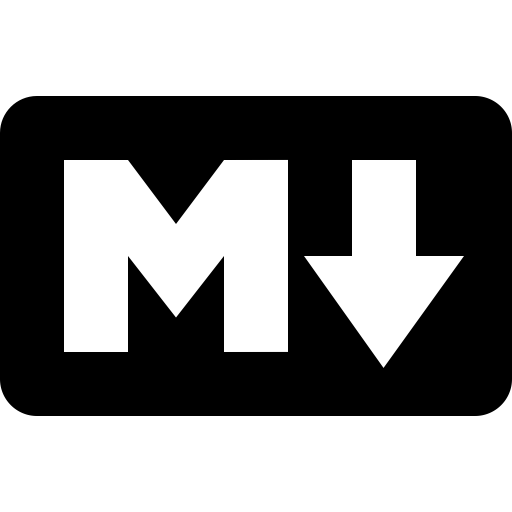
\includegraphics[scale=0.2]{imagenes/markdown-512.png} 
\end{center}
\end{frame}

\section{Comparación entre Latex y Markdown}

\begin{frame}{Comparación entre Latex y Markdown}
\begin{center}
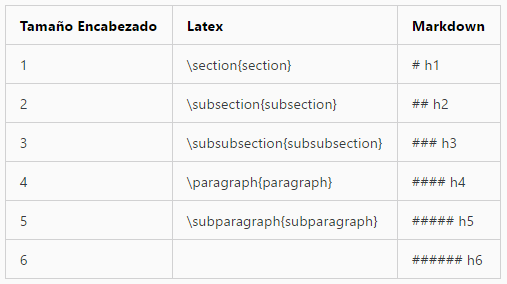
\includegraphics[scale=0.8]{imagenes/com.png} 
\end{center}
\end{frame}

\begin{frame}
\begin{center}
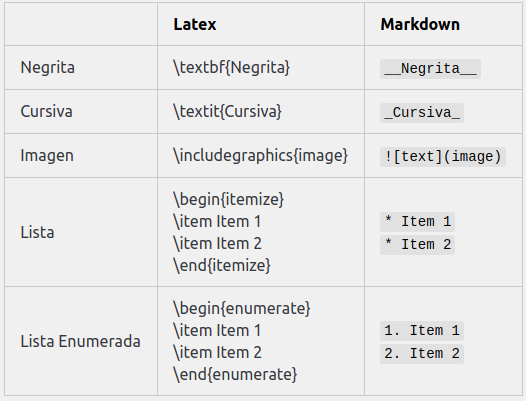
\includegraphics[scale=0.6]{imagenes/table.png} 
\end{center}
\end{frame}




\begin{frame}[fragile]

\textbf{Codigo en markdown}

%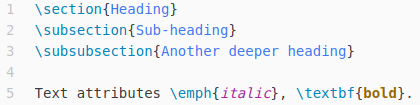
\includegraphics[scale=.7]{imagenes/la.png} \\

\begin{minted}{python}
# Heading
## Sub-heading
### Another deeper heading
 
Text attributes _italic_, __bold__.

\end{minted}


\vspace{1cm}
\textbf{Codigo en \LaTeX}
%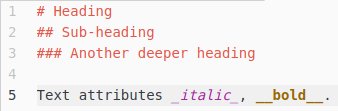
\includegraphics[scale=.7]{imagenes/md.png} 


\begin{minted}{latex}
\section{Heading}
\subsection{Sub-heading}
\subsubsection{Another deeper heading}\

Text attributes \emph{italic}, \textbf{bold}.

\end{minted}

\end{frame}

\section{Análisis léxico}

\subsection{Tabla de tokens}

\begin{frame}{Análisis léxico}{Tabla de tokens}

\begin{center}
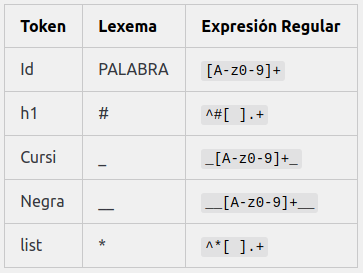
\includegraphics[scale=0.7]{imagenes/lex.png} 
\end{center}
\end{frame}

\subsection{Automatas}

\begin{frame}[fragile]{Automata para las cabeceras}
\begin{center}
\begin{tikzpicture}[scale=0.2]

\tikzstyle{every node}+=[inner sep=0pt]
\draw [black] (11.2,-28.4) circle (3);
\draw (11.2,-28.4) node {$1$};
\draw [black] (20.8,-17.3) circle (3);
\draw (20.8,-17.3) node {$2$};
\draw [black] (40.1,-14.7) circle (3);
\draw (40.1,-14.7) node {$3$};
\draw [black] (59.5,-17) circle (3);
\draw (59.5,-17) node {$4$};
\draw [black] (38.5,-37.8) circle (3);
\draw (38.5,-37.8) node {$5$};
\draw [black] (63.3,-39.4) circle (3);
\draw (63.3,-39.4) node {$6$};
\draw [black] (63.3,-39.4) circle (2.4);
\draw [black] (13.16,-26.13) -- (18.84,-19.57);
\fill [black] (18.84,-19.57) -- (17.94,-19.85) -- (18.69,-20.5);
\draw (16.55,-24.3) node [right] {$\#$};
\draw [black] (23.77,-16.9) -- (37.13,-15.1);
\fill [black] (37.13,-15.1) -- (36.27,-14.71) -- (36.4,-15.7);
\draw (30.76,-16.59) node [below] {$\#$};
\draw [black] (43.08,-15.05) -- (56.52,-16.65);
\fill [black] (56.52,-16.65) -- (55.79,-16.06) -- (55.67,-17.05);
\draw (49.55,-16.44) node [below] {$\#$};
\draw [black] (22.76,-19.57) -- (36.54,-35.53);
\fill [black] (36.54,-35.53) -- (36.4,-34.6) -- (35.64,-35.25);
\draw (29.1,-29) node [left] {$\setminus s$};
\draw [black] (39.89,-17.69) -- (38.71,-34.81);
\fill [black] (38.71,-34.81) -- (39.26,-34.04) -- (38.26,-33.97);
\draw (38.7,-26.21) node [left] {$\setminus s$};
\draw [black] (57.37,-19.11) -- (40.63,-35.69);
\fill [black] (40.63,-35.69) -- (41.55,-35.48) -- (40.85,-34.77);
\draw (47.81,-26.92) node [above] {$\setminus s$};
\draw [black] (41.49,-37.99) -- (60.31,-39.21);
\fill [black] (60.31,-39.21) -- (59.54,-38.66) -- (59.48,-39.65);
\draw (50.79,-39.18) node [below] {$\setminus n$};
\draw [black] (38.809,-40.772) arc (33.67686:-254.32314:2.25);
\draw (34.08,-44.69) node [below] {$char$};
\fill [black] (36.33,-39.85) -- (35.39,-39.88) -- (35.94,-40.71);
\end{tikzpicture}
\end{center}

\end{frame}

\begin{frame}[fragile]{Automata para la negrita y la cursiva}

\begin{center}
\begin{tikzpicture}[scale=0.15]
\tikzstyle{every node}+=[inner sep=0pt]
\draw [black] (8.7,-34) circle (3);
\draw (8.7,-34) node {$7$};
\draw [black] (26.8,-17.3) circle (3);
\draw (26.8,-17.3) node {$8$};
\draw [black] (46.9,-17.3) circle (3);
\draw (46.9,-17.3) node {$9$};
\draw [black] (62.3,-17.3) circle (3);
\draw (62.3,-17.3) node {$10$};
\draw [black] (62.3,-17.3) circle (2.4);
\draw [black] (26.8,-39.4) circle (3);
\draw (26.8,-39.4) node {$11$};
\draw [black] (40.6,-39.8) circle (3);
\draw (40.6,-39.8) node {$12$};
\draw [black] (54.4,-39.8) circle (3);
\draw (54.4,-39.8) node {$13$};
\draw [black] (69.9,-39.8) circle (3);
\draw (69.9,-39.8) node {$14$};
\draw [black] (69.9,-39.8) circle (2.4);
\draw [black] (10.9,-31.97) -- (24.6,-19.33);
\fill [black] (24.6,-19.33) -- (23.67,-19.51) -- (24.35,-20.24);
\draw (18.6,-26.14) node [below] {$-$};
\draw [black] (29.8,-17.3) -- (43.9,-17.3);
\fill [black] (43.9,-17.3) -- (43.1,-16.8) -- (43.1,-17.8);
\draw (36.85,-17.8) node [below] {$char$};
\draw [black] (45.577,-14.62) arc (234:-54:2.25);
\draw (46.9,-10.05) node [above] {$char$};
\fill [black] (48.22,-14.62) -- (49.1,-14.27) -- (48.29,-13.68);
\draw [black] (49.9,-17.3) -- (59.3,-17.3);
\fill [black] (59.3,-17.3) -- (58.5,-16.8) -- (58.5,-17.8);
\draw (54.6,-17.8) node [below] {$-$};
\draw [black] (26.8,-20.3) -- (26.8,-36.4);
\fill [black] (26.8,-36.4) -- (27.3,-35.6) -- (26.3,-35.6);
\draw (26.3,-28.35) node [left] {$-$};
\draw [black] (29.8,-39.49) -- (37.6,-39.71);
\fill [black] (37.6,-39.71) -- (36.82,-39.19) -- (36.79,-40.19);
\draw (33.66,-40.16) node [below] {$char$};
\draw [black] (42.272,-42.276) arc (61.76517:-226.23483:2.25);
\draw (42.22,-47.19) node [below] {$char$};
\fill [black] (39.65,-42.63) -- (38.83,-43.1) -- (39.71,-43.58);
\draw [black] (43.6,-39.8) -- (51.4,-39.8);
\fill [black] (51.4,-39.8) -- (50.6,-39.3) -- (50.6,-40.3);
\draw (47.5,-40.3) node [below] {$-$};
\draw [black] (57.4,-39.8) -- (66.9,-39.8);
\fill [black] (66.9,-39.8) -- (66.1,-39.3) -- (66.1,-40.3);
\draw (62.15,-40.3) node [below] {$-$};
\end{tikzpicture}
\end{center}
\end{frame}


\begin{frame}[fragile]{Automata final}

\begin{center}

\begin{center}
\begin{tikzpicture}[scale=0.15]
\tikzstyle{every node}+=[inner sep=0pt]
\draw [black] (36,-28.9) circle (3);
\draw (36,-28.9) node {$1$};
\draw [black] (36,-28.9) circle (2.4);
\draw [black] (36,-13.9) circle (3);
\draw (36,-13.9) node {$2$};
\draw [black] (22.2,-13.9) circle (3);
\draw (22.2,-13.9) node {$3$};
\draw [black] (49.4,-13.9) circle (3);
\draw (49.4,-13.9) node {$5$};
\draw [black] (61.3,-13.9) circle (3);
\draw (61.3,-13.9) node {$6$};
\draw [black] (73.7,-13.9) circle (3);
\draw (73.7,-13.9) node {$7$};
\draw [black] (36,-38.7) circle (3);
\draw (36,-38.7) node {$8$};
\draw [black] (36,-51.4) circle (3);
\draw (36,-51.4) node {$9$};
\draw [black] (56.2,-51.4) circle (3);
\draw (56.2,-51.4) node {$10$};
\draw [black] (56.2,-38.7) circle (3);
\draw (56.2,-38.7) node {$11$};
\draw [black] (29.1,-28.9) -- (33,-28.9);
\fill [black] (33,-28.9) -- (32.2,-28.4) -- (32.2,-29.4);
\draw [black] (36,-25.9) -- (36,-16.9);
\fill [black] (36,-16.9) -- (35.5,-17.7) -- (36.5,-17.7);
\draw (36.5,-21.4) node [right] {$-$};
\draw [black] (33,-13.9) -- (25.2,-13.9);
\fill [black] (25.2,-13.9) -- (26,-14.4) -- (26,-13.4);
\draw (29.1,-13.4) node [above] {$char$};
\draw [black] (39,-13.9) -- (46.4,-13.9);
\fill [black] (46.4,-13.9) -- (45.6,-13.4) -- (45.6,-14.4);
\draw (42.7,-14.4) node [below] {$-$};
\draw [black] (52.4,-13.9) -- (58.3,-13.9);
\fill [black] (58.3,-13.9) -- (57.5,-13.4) -- (57.5,-14.4);
\draw (55.35,-14.4) node [below] {$char$};
\draw [black] (21.458,-11.005) arc (222.11134:-65.88866:2.25);
\draw (24.92,-6.61) node [above] {$char$};
\fill [black] (24.05,-11.55) -- (24.97,-11.38) -- (24.3,-10.64);
\draw [black] (61.564,-10.923) arc (202.67131:-85.32869:2.25);
\draw (67.03,-7.63) node [above] {$char$};
\fill [black] (63.82,-12.3) -- (64.75,-12.45) -- (64.37,-11.53);
\draw [black] (64.3,-13.9) -- (70.7,-13.9);
\fill [black] (70.7,-13.9) -- (69.9,-13.4) -- (69.9,-14.4);
\draw (67.5,-14.4) node [below] {$-$};
\draw [black] (70.91,-15.01) -- (38.79,-27.79);
\fill [black] (38.79,-27.79) -- (39.72,-27.96) -- (39.35,-27.03);
\draw (55.64,-21.92) node [below] {$-$};
\draw [black] (36,-31.9) -- (36,-35.7);
\fill [black] (36,-35.7) -- (36.5,-34.9) -- (35.5,-34.9);
\draw (36.5,-33.8) node [right] {$\#$};
\draw [black] (36,-41.7) -- (36,-48.4);
\fill [black] (36,-48.4) -- (36.5,-47.6) -- (35.5,-47.6);
\draw (35.5,-45.05) node [left] {$\#$};
\draw [black] (39,-51.4) -- (53.2,-51.4);
\fill [black] (53.2,-51.4) -- (52.4,-50.9) -- (52.4,-51.9);
\draw (46.1,-51.9) node [below] {$\#$};
\draw [black] (39,-38.7) -- (53.2,-38.7);
\fill [black] (53.2,-38.7) -- (52.4,-38.2) -- (52.4,-39.2);
\draw (46.1,-38.2) node [above] {$\setminus s$};
\draw [black] (56.2,-48.4) -- (56.2,-41.7);
\fill [black] (56.2,-41.7) -- (55.7,-42.5) -- (56.7,-42.5);
\draw (56.7,-45.05) node [right] {$\setminus s$};
\draw [black] (38.54,-49.8) -- (53.66,-40.3);
\fill [black] (53.66,-40.3) -- (52.72,-40.3) -- (53.25,-41.15);
\draw (46.99,-45.55) node [below] {$\setminus s$};
\draw [black] (59.065,-37.851) arc (134.23913:-153.76087:2.25);
\draw (63.57,-40.09) node [right] {$char$};
\fill [black] (58.62,-40.46) -- (58.82,-41.38) -- (59.53,-40.68);
\draw [black] (53.5,-37.39) -- (38.7,-30.21);
\fill [black] (38.7,-30.21) -- (39.2,-31.01) -- (39.64,-30.11);
\draw (47.09,-33.29) node [above] {$\setminus n$};
\draw [black] (34.851,-31.659) arc (5.12592:-282.87408:2.25);
\draw (30.37,-34.79) node [left] {$Any$};
\fill [black] (33.11,-29.67) -- (32.27,-29.24) -- (32.36,-30.24);
\draw [black] (24.23,-16.11) -- (33.97,-26.69);
\fill [black] (33.97,-26.69) -- (33.8,-25.76) -- (33.06,-26.44);
\draw (28.57,-22.86) node [left] {$-$};
\end{tikzpicture}
\end{center}
\end{center}

\end{frame}

\subsection{Código en C}

\begin{frame}[fragile]{Código en C}

\begin{center}
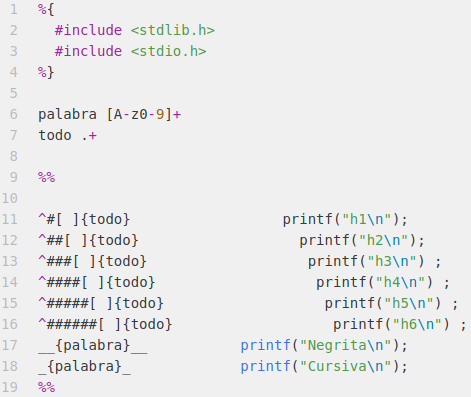
\includegraphics[scale=0.55]{imagenes/code.png} 

\end{center}
\end{frame}


\section{Análisis sintactico}

\begin{frame}[fragile]{Análisis sintactico}{Su gramatica libre de contexto es}
\begin{minted}{python}
A-> h1 | h2 | h3 | N | C | B | A | \n
h1 -> # \s B \n A
h2 -> ## \s B \n A
h3 -> ### \s B \n A
N -> _B_A
C -> __B__A
B -> a|b|...|z|0|...|9|\t|BB| A 
\end{minted}
\end{frame}

\end{document}
